\documentclass[a4paper,10pt]{jsarticle}

% 数式
\usepackage{amsmath,amsfonts}
\usepackage{bm}
% 画像
\usepackage[dvipdfmx]{graphicx}
\usepackage{here}

\usepackage{listingsutf8,jlisting} %日本語のコメントアウトをする場合jlistingが必要
%ここからソースコードの表示に関する設定
\lstset{
  basicstyle={\ttfamily},
  identifierstyle={\small},
  commentstyle={\smallitshape},
  keywordstyle={\small\bfseries},
  ndkeywordstyle={\small},
  stringstyle={\small\ttfamily},
  frame={tb},
  breaklines=true,
  columns=[l]{fullflexible},
  numbers=left,
  xrightmargin=0zw,
  xleftmargin=3zw,
  numberstyle={\scriptsize},
  stepnumber=1,
  numbersep=1zw,
  lineskip=-0.5ex
}

\begin{document}

\title{データベース2演習課題2}
\author{坪井正太郎(101830245)}
\date{\today}
\maketitle
\section{}
\[\pi_{タイトル, 監督名, 氏名}(\sigma_{映画.映画ID=出演.映画ID\wedge  俳優.俳優ID=出演.俳優ID\wedge 国籍='日本'\wedge 年='2000'}(映画\times 出演\times 俳優))\]

\section{}
\begin{figure}[H]
  \centering
  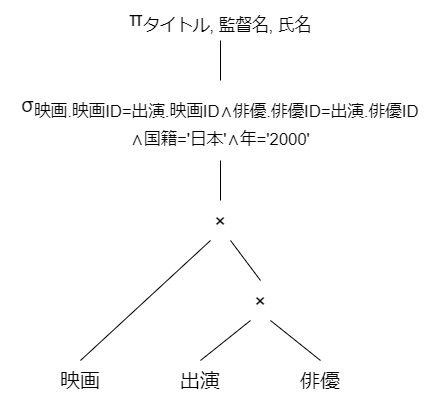
\includegraphics[width=12cm]{01.drawio.png}
  \caption{処理木}
  \label{処理木}
\end{figure}

\section{}
NATURAL JOINは記号$\Join$として扱う。
\begin{figure}[H]
  \centering
  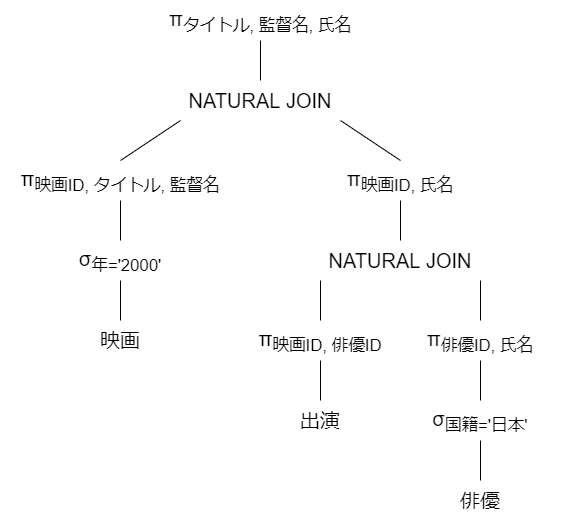
\includegraphics[width=12cm]{02.drawio.png}
  \caption{変換後の処理木}
  \label{変換後の処理木}
\end{figure}

\end{document}
